\documentclass[12pt,a4paper]{article}

% ── Packages ─────────────────────────────────────────────────────────────────
\usepackage[a4paper, margin=2.5cm]{geometry}
\usepackage{graphicx}
\usepackage{booktabs}
\usepackage{longtable}
\usepackage{array}
\usepackage{xcolor}
\PassOptionsToPackage{hyphens}{url}
\usepackage{hyperref}
\usepackage{enumitem}
\usepackage{titlesec}
\usepackage{fancyhdr}
\usepackage{tikz}
\usepackage{amsmath}
\usepackage{listings}
\usepackage{microtype}
\usepackage{parskip}
\usepackage{float}
\usepackage{caption}
\usepackage{subcaption}
\usepackage{tabularx}
\usepackage{multirow}
\usepackage{adjustbox}

\usetikzlibrary{shapes.geometric, arrows.meta, positioning, fit, backgrounds,
                shapes.symbols, calc, decorations.pathreplacing}

% ── Colours ──────────────────────────────────────────────────────────────────
\definecolor{accent}{HTML}{2563EB}
\definecolor{lightgray}{HTML}{F3F4F6}
\definecolor{darkgray}{HTML}{374151}
\definecolor{bpmngreen}{HTML}{22C55E}
\definecolor{bpmnblue}{HTML}{3B82F6}
\definecolor{bpmnorange}{HTML}{F59E0B}
\definecolor{bpmnred}{HTML}{EF4444}
\definecolor{codebg}{HTML}{F8F9FA}

% ── Hyperref setup ───────────────────────────────────────────────────────────
\hypersetup{
  colorlinks=true, linkcolor=accent, urlcolor=accent, citecolor=accent,
  pdftitle={allStay HMS Design Report}, pdfauthor={Team allStay}
}

% ── Code listings ────────────────────────────────────────────────────────────
\lstset{
  backgroundcolor=\color{codebg},
  basicstyle=\ttfamily\footnotesize,
  breaklines=true, frame=single, rulecolor=\color{lightgray},
  numbers=left, numberstyle=\tiny\color{darkgray},
  showstringspaces=false, tabsize=2
}

% ── Section formatting ───────────────────────────────────────────────────────
\titleformat{\section}{\large\bfseries\color{accent}}{}{0em}{}[\vspace{-0.3em}\rule{\linewidth}{0.8pt}]
\titleformat{\subsection}{\normalsize\bfseries\color{darkgray}}{}{0em}{}

% ── Headers / Footers ────────────────────────────────────────────────────────
\pagestyle{fancy}
\fancyhf{}
\fancyhead[L]{\small\color{darkgray}allStay Hotel Management System}
\fancyhead[R]{\small\color{darkgray}Database Application and Design --- Spring 2026}
\fancyfoot[C]{\thepage}
\renewcommand{\headrulewidth}{0.4pt}

% ── TikZ styles ──────────────────────────────────────────────────────────────
\tikzset{
  % ER entities
  entity/.style={rectangle, draw=accent, fill=accent!10, rounded corners=3pt,
                 minimum width=2.4cm, minimum height=0.65cm,
                 font=\scriptsize\bfseries, text=accent, align=center},
  % ER relationship lines
  rel/.style={draw=darkgray!70, thick},
  % BPMN shapes
  bstart/.style={circle, draw=bpmngreen!80!black, fill=bpmngreen!25,
                 minimum size=0.65cm, font=\tiny\bfseries},
  bend/.style={circle, double, draw=bpmnred!80!black, fill=bpmnred!15,
               minimum size=0.65cm},
  btask/.style={rectangle, draw=bpmnblue!80!black, fill=bpmnblue!10,
                rounded corners=3pt, minimum width=2.2cm, minimum height=0.75cm,
                font=\scriptsize, align=center, text width=2.2cm},
  bgate/.style={diamond, draw=bpmnorange!80!black, fill=bpmnorange!15,
                minimum size=0.65cm, font=\tiny, aspect=1.8},
  barrow/.style={->, >=Stealth, draw=darkgray, thick},
  % Architecture service boxes — usage: \node[svc=accent] ...
  svc/.style={rectangle, draw=#1, fill=#1!12, rounded corners=4pt,
              minimum width=2.6cm, minimum height=0.8cm,
              font=\scriptsize\bfseries, align=center, text=#1},
}

% ─────────────────────────────────────────────────────────────────────────────
\begin{document}
\thispagestyle{empty}

% ══════════════════════════════════════════════════════════════════════════════
%  COVER PAGE
% ══════════════════════════════════════════════════════════════════════════════
\begin{titlepage}
\centering
\vspace*{1.2cm}

{\Huge\bfseries\color{accent} allStay}\\[0.4em]
{\Large Hotel Management System}\\[0.25em]
{\normalsize\itshape\color{darkgray} ``Every stay, seamlessly managed.''}

\vspace{1.6cm}
\rule{\linewidth}{1pt}\\[0.4em]
{\large\bfseries Database Application and Design --- Group Project}\\
{\normalsize Spring 2026 \quad|\quad Inha University in Tashkent}\\[0.4em]
\rule{\linewidth}{0.4pt}

\vspace{1.8cm}
{\large\bfseries Team Members}

\vspace{0.6em}
\begin{tabular}{@{}lll@{}}
\toprule
\textbf{Name} & \textbf{Student ID} & \textbf{Role} \\
\midrule
Axmadov Sunnat          & U2310044 & Team Lead $\cdot$ Backend Architecture \\
Mirshod Hamroyev        & U2310088 & Backend API \& Authentication \\
Nurmuhammad Fazliddinov & U2310082 & Database Design \& Migrations \\
Hamidov Abror           & U2310087 & DevOps \& Infrastructure \\
Yusufova Muxlisa        & U2310298 & Frontend \& UI Design \\
Izbosarov Bekzod        & U2310113 & Observability \& Testing \\
\bottomrule
\end{tabular}

\vspace{1.8cm}
\begin{tabular}{@{}ll@{}}
\textbf{GitHub Repository:} & \url{https://github.com/Uzsoftdev/hotel_ms} \\[0.4em]
\textbf{Deployed URL:}       & \url{https://allstay.rest} \\[0.4em]
\textbf{Date:}               & 17 May 2026 \\
\end{tabular}

\vfill
{\small Submitted to \textbf{eclass.inha.ac.kr} by team leader Axmadov Sunnat}
\end{titlepage}

\newpage
\setcounter{page}{1}

% ══════════════════════════════════════════════════════════════════════════════
%  ABSTRACT
% ══════════════════════════════════════════════════════════════════════════════
\section*{Abstract}
\addcontentsline{toc}{section}{Abstract}

allStay is a full-stack distributed hotel management system designed to serve guests, hotel staff, and administrators through a unified platform. Guests can search and book rooms, make payments, and receive real-time booking updates via WebSocket. Staff can manage check-ins, room status, and guest requests. Administrators have full control over room inventory, dynamic pricing, user accounts, and business analytics reports.

The backend is built on \textbf{FastAPI} with a \textbf{PostgreSQL~15} primary database, a hot-standby streaming replica, and \textbf{PgBouncer} for connection pooling. \textbf{Redis} serves triple duty as an availability cache, Celery task broker, and token-bucket state store. \textbf{Meilisearch} provides millisecond full-text hotel and room search. Files (avatars, hotel images) are stored in \textbf{MinIO} (S3-compatible). Two FastAPI replicas sit behind a \textbf{Traefik~v3.1} API gateway with TLS termination and load balancing. A \textbf{Celery Beat} scheduler drives nightly revenue aggregation and hourly cache warm-up. A token-bucket rate limiter---implemented from scratch using Redis Lua scripts---protects all endpoints. The entire stack is observable through \textbf{Prometheus}, \textbf{Grafana}, \textbf{Loki}, and \textbf{Jaeger} via OpenTelemetry.

% ══════════════════════════════════════════════════════════════════════════════
%  1. BUSINESS REQUIREMENTS
% ══════════════════════════════════════════════════════════════════════════════
\section{Business Requirements}

\subsection{Scenario}
allStay is a Software-as-a-Service hotel management platform built for boutique hotel chains. It replaces paper-based check-in registers and disconnected spreadsheet pricing with a single web interface and a real-time API, allowing hotels to maximise occupancy and deliver a modern guest experience.

\subsection{Use Cases}

\begin{enumerate}[leftmargin=*, label=\textbf{UC\arabic*.}]

\item \textbf{Guest Books a Room} ---
  \textit{Actor:} Registered guest. \quad
  \textit{Flow:} Search hotels by city and dates $\to$ browse rooms with filters $\to$ select room $\to$ choose dates $\to$ submit booking $\to$ payment recorded $\to$ confirmation email sent $\to$ real-time WebSocket notification pushed.

\item \textbf{Staff Processes Check-In} ---
  \textit{Actor:} Hotel staff. \quad
  \textit{Flow:} Open daily assigned bookings $\to$ identify arriving guest $\to$ verify identity $\to$ mark booking \texttt{checked\_in} via admin API $\to$ system pushes WebSocket notification to the guest's connected client.

\item \textbf{Admin Configures Dynamic Pricing} ---
  \textit{Actor:} Hotel administrator. \quad
  \textit{Flow:} Create pricing rule (date range, day-of-week, fixed price or multiplier) $\to$ rule persisted $\to$ availability queries apply the rule immediately.

\item \textbf{System Runs Nightly Revenue Snapshot} ---
  \textit{Actor:} System (Celery Beat). \quad
  \textit{Flow:} At 02:00~UTC Celery Beat triggers \texttt{nightly\_revenue\_snapshot} $\to$ query non-cancelled bookings from yesterday $\to$ aggregate by room type $\to$ write summary to \texttt{activity\_logs} $\to$ log completion.

\item \textbf{Guest Receives Real-Time Notification} ---
  \textit{Actor:} Guest (connected via WebSocket). \quad
  \textit{Flow:} Booking status changes $\to$ backend publishes to Redis Pub/Sub channel $\to$ all backend replicas receive message $\to$ correct replica delivers payload to the connected browser.

\item \textbf{Admin Reviews Revenue Reports} ---
  \textit{Actor:} Hotel administrator. \quad
  \textit{Flow:} Open Reports panel $\to$ select date range $\to$ backend queries \texttt{activity\_logs} and live bookings $\to$ returns occupancy rate, revenue per room type, and guest demographics.

\end{enumerate}

\subsection{Functional Requirements}
\begin{itemize}[noitemsep]
  \item Guest registration, login (email/password and Google OAuth~2.0), email verification, and password reset.
  \item Full RBAC: \texttt{guest}, \texttt{staff}, \texttt{hotel\_admin}, \texttt{super\_admin}.
  \item Room and hotel search with filters (city, price range, capacity, amenities, dates).
  \item Real-time availability check with Redis caching.
  \item End-to-end booking flow: create $\to$ confirm $\to$ check-in $\to$ check-out.
  \item Dynamic pricing rules (fixed price or multiplier, date range, day-of-week, priority).
  \item Review and rating system (one review per completed booking).
  \item Wishlist / saved rooms per guest.
  \item Real-time notifications via WebSocket.
  \item Admin dashboard: room management, booking oversight, user/staff management, reports.
  \item Staff dashboard: assigned bookings, check-in/out, task management, room status board.
\end{itemize}

\subsection{Non-Functional Requirements}

% FIX: replaced broken tabularx with fixed-width p{} columns and concise text
\begin{table}[H]
\centering\small
\begin{tabular}{@{} p{2.2cm} p{4.8cm} p{5.6cm} @{}}
\toprule
\textbf{Quality} & \textbf{Target / SLA} & \textbf{Mechanism} \\
\midrule
Availability  & $>$99.9\% uptime                       & 2 backend replicas; Traefik circuit breaker \\[4pt]
Latency       & p95 API $<$200 ms; cached $<$10 ms     & Redis availability cache; PgBouncer pooling \\[4pt]
Throughput    & 200 req/min per IP (auth: 10--20/min)  & Token-bucket rate limiter (R11) \\[4pt]
Security      & TLS everywhere; JWT expiry; RBAC       & Traefik + Let's Encrypt; middleware chain \\[4pt]
Scalability   & Horizontal backend scale-out           & Stateless replicas; Docker Compose \\
\midrule
\multicolumn{3}{@{}l@{}}{\textbf{Scale assumptions:} 1\,000 concurrent users; 50 hotels; 500+ rooms; 10\,000+ bookings/month} \\
\bottomrule
\end{tabular}
\end{table}

% ══════════════════════════════════════════════════════════════════════════════
%  2. DOMAIN MODEL AND ER DIAGRAM
% ══════════════════════════════════════════════════════════════════════════════
\section{Domain Model and ER Diagram}

\subsection{Entity Inventory}

The relational schema comprises \textbf{20 tables}. Key entities are described below.

\begin{table}[H]
\centering\small
\begin{tabularx}{\linewidth}{lX}
\toprule
\textbf{Entity} & \textbf{Key Attributes} \\
\midrule
\texttt{users}        & id, email, password\_hash, first\_name, last\_name, phone, role (ENUM), hotel\_id (FK), avatar\_url, is\_active \\
\texttt{hotels}       & id, name, city, country, address, description, star\_rating (1--5), is\_active \\
\texttt{room\_types}  & id, hotel\_id (FK), name, description, base\_price, capacity \\
\texttt{rooms}        & id, hotel\_id (FK), room\_type\_id (FK), room\_number, floor, is\_active \\
\texttt{bookings}     & id, user\_id (FK), room\_id (FK), check\_in, check\_out, guests, total\_price, status (ENUM: pending / confirmed / cancelled / completed) \\
\texttt{payments}     & id, booking\_id (FK), amount, currency, method, status, transaction\_id \\
\texttt{pricing\_rules} & id, hotel\_id (FK), room\_type\_id (FK), priority, rule\_type (fixed / multiplier), value, start\_date, end\_date, day\_of\_week \\
\texttt{blackout\_dates} & id, hotel\_id (FK), date, reason \\
\texttt{reviews}      & id, user\_id (FK), booking\_id (FK), hotel\_id (FK), rating (1--5), comment \\
\texttt{notifications} & id, user\_id (FK), type, message, is\_read, created\_at \\
\texttt{activity\_logs} & id, user\_id (FK, nullable), action, resource, detail, created\_at \\
\texttt{wishlists}    & id, user\_id (FK), hotel\_id (FK) \\
\texttt{amenities}    & id, name, icon \\
\texttt{facilities}   & id, name, icon \\
\texttt{hotel\_facilities} & hotel\_id (FK), facility\_id (FK) --- junction \\
\texttt{hotel\_images}  & id, hotel\_id (FK), url, is\_primary \\
\texttt{room\_images}   & id, room\_id (FK), url, is\_primary \\
\texttt{room\_amenities} & room\_id (FK), amenity\_id (FK) --- junction \\
\texttt{email\_verifications} & id, user\_id (FK), token, expires\_at \\
\texttt{password\_resets} & id, user\_id (FK), token, expires\_at \\
\bottomrule
\end{tabularx}
\end{table}

\clearpage
\subsection{ER Diagram}

The diagram shows the principal entities and their relationships. Cardinalities are annotated on each line. Junction tables (\texttt{room\_amenities}, \texttt{hotel\_facilities}) represent M:N associations.

% FIX: use explicit (x,y) absolute coordinates so nodes never overlap
\begin{figure}[H]
\centering
\begin{adjustbox}{max width=\linewidth, max totalheight=0.80\textheight, keepaspectratio}
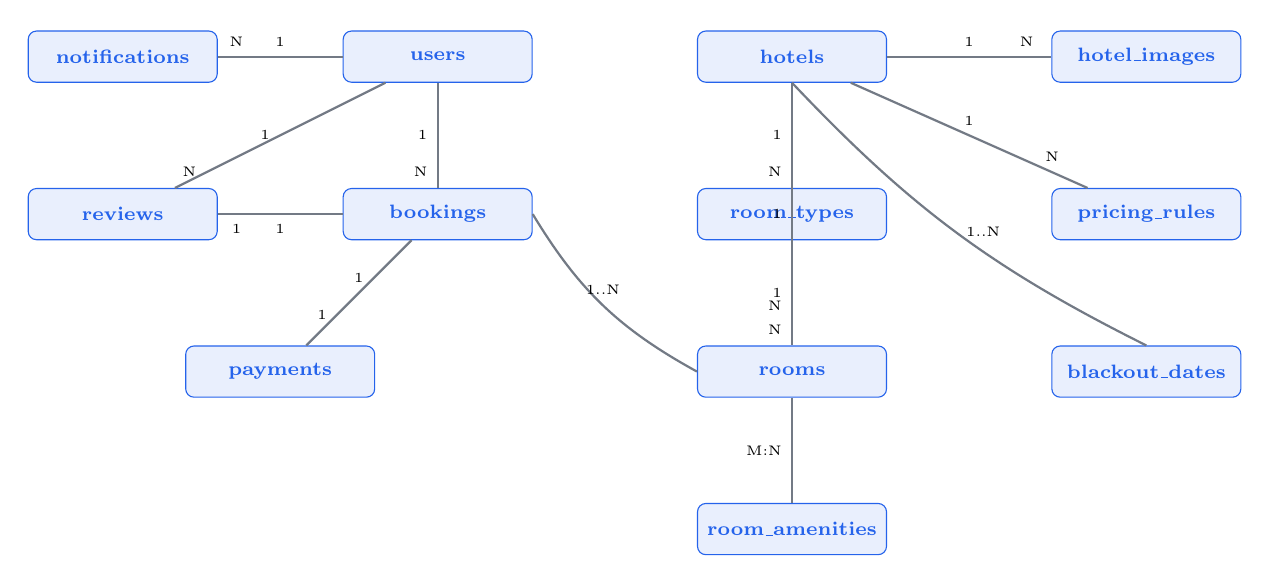
\begin{tikzpicture}[font=\scriptsize]

% ── Row 3 (y=4) ──────────────────────────────────────────────────────────────
\node[entity] (notif)   at (0,   4)  {notifications};
\node[entity] (user)    at (4,   4)  {users};
\node[entity] (hotel)   at (8.5, 4)  {hotels};
\node[entity] (himage)  at (13,  4)  {hotel\_images};

% ── Row 2 (y=2) ──────────────────────────────────────────────────────────────
\node[entity] (review)  at (0,   2)  {reviews};
\node[entity] (booking) at (4,   2)  {bookings};
\node[entity] (rtype)   at (8.5, 2)  {room\_types};
\node[entity] (pricing) at (13,  2)  {pricing\_rules};

% ── Row 1 (y=0) ──────────────────────────────────────────────────────────────
\node[entity] (payment) at (2,   0)  {payments};
\node[entity] (room)    at (8.5, 0)  {rooms};
\node[entity] (blackout)at (13,  0)  {blackout\_dates};

% ── Row 0 (y=-2) ─────────────────────────────────────────────────────────────
\node[entity] (ramen)   at (8.5, -2) {room\_amenities};

% ── Relationships ─────────────────────────────────────────────────────────────
% users - notifications (1:N)
\draw[rel] (user) -- node[above,font=\tiny]{1} (notif)
  node[pos=0.85,above,font=\tiny]{N};

% users - reviews (1:N)
\draw[rel] (user) -- node[left,font=\tiny]{1}
  node[pos=0.85,left,font=\tiny]{N} (review);

% users - bookings (1:N)
\draw[rel] (user) -- node[left,font=\tiny]{1}
  node[pos=0.85,left,font=\tiny]{N} (booking);

% hotels - hotel_images (1:N)
\draw[rel] (hotel) -- node[above,font=\tiny]{1}
  node[pos=0.85,above,font=\tiny]{N} (himage);

% hotels - room_types (1:N)
\draw[rel] (hotel) -- node[left,font=\tiny]{1}
  node[pos=0.85,left,font=\tiny]{N} (rtype);

% hotels - pricing_rules (1:N)
\draw[rel] (hotel) -- node[above,font=\tiny]{1}
  node[pos=0.85,above,font=\tiny]{N} (pricing);

% hotels - blackout_dates (1:N)
\draw[rel] (hotel.south) to[bend right=10]
  node[right,font=\tiny]{1..N} (blackout.north);

% hotels - rooms (1:N) via a bend
\draw[rel] (hotel.south) -- node[left,font=\tiny]{1}
  node[pos=0.85,left,font=\tiny]{N} (room.north);

% room_types - rooms (1:N)
\draw[rel] (rtype) -- node[left,font=\tiny]{1}
  node[pos=0.85,left,font=\tiny]{N} (room);

% rooms - room_amenities (1:N -> M:N junction)
\draw[rel] (room) -- node[left,font=\tiny]{M:N} (ramen);

% bookings - payments (1:1)
\draw[rel] (booking) -- node[above,font=\tiny]{1}
  node[pos=0.85,above,font=\tiny]{1} (payment);

% bookings - reviews (1:1)
\draw[rel] (booking) -- node[below,font=\tiny]{1}
  node[pos=0.85,below,font=\tiny]{1} (review);

% rooms - bookings (1:N)
\draw[rel] (room.west) to[bend left=15]
  node[above,font=\tiny]{1..N} (booking.east);

\end{tikzpicture}
\end{adjustbox}
\caption{ER diagram --- 20-table schema (junction tables shown as M:N labels)}
\end{figure}

% ══════════════════════════════════════════════════════════════════════════════
%  3. SYSTEM ARCHITECTURE
% ══════════════════════════════════════════════════════════════════════════════
\clearpage
\section{System Architecture}

% FIX: all nodes use explicit (x,y) coordinates to eliminate any overlap
\begin{figure}[H]
\centering
\begin{adjustbox}{max width=\linewidth, max totalheight=0.72\textheight, keepaspectratio}
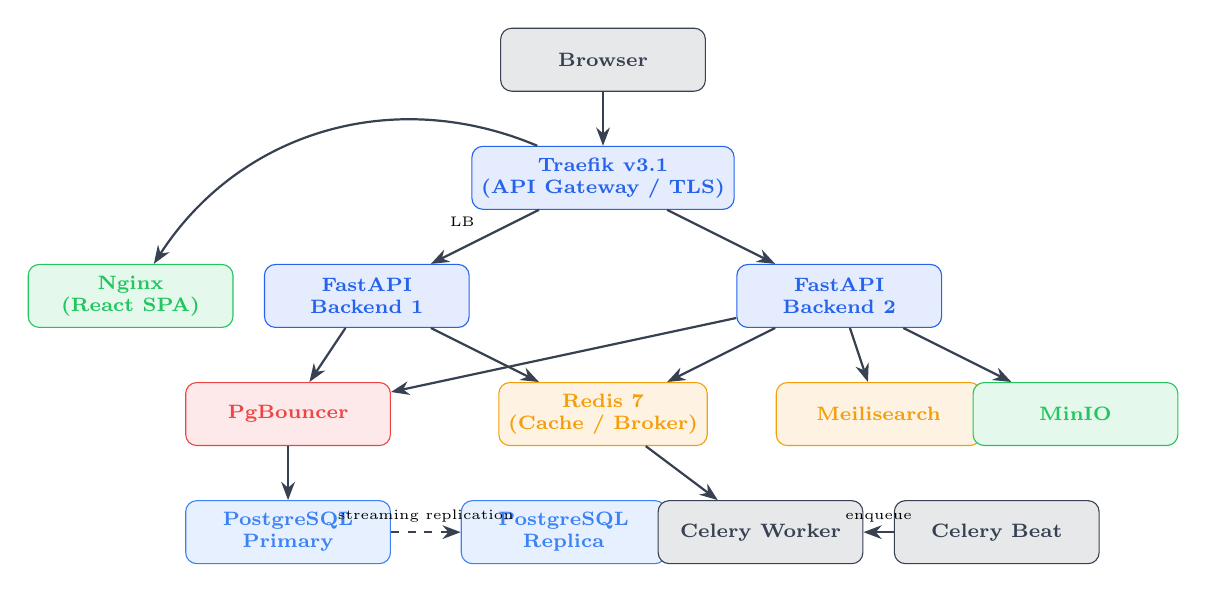
\begin{tikzpicture}[font=\scriptsize, node distance=0pt]

% ── Row 1: Browser ───────────────────────────────────────────────────────────
\node[svc=darkgray] (browser) at (6, 8.5) {Browser};

% ── Row 2: Gateway ───────────────────────────────────────────────────────────
\node[svc=accent]   (traefik) at (6, 7.0)
  {Traefik v3.1\\(API Gateway / TLS)};

% ── Row 3: Backend replicas + Nginx ──────────────────────────────────────────
\node[svc=accent]       (be1)   at (3,   5.5) {FastAPI\\Backend 1};
\node[svc=accent]       (be2)   at (9,   5.5) {FastAPI\\Backend 2};
\node[svc=bpmngreen]    (nginx) at (0,   5.5) {Nginx\\(React SPA)};

% ── Row 4: Data / storage layer ──────────────────────────────────────────────
\node[svc=bpmnred]      (pgb)   at (2,   4.0) {PgBouncer};
\node[svc=bpmnorange]   (redis) at (6,   4.0) {Redis 7\\(Cache / Broker)};
\node[svc=bpmnorange]   (meili) at (9.5, 4.0) {Meilisearch};
\node[svc=bpmngreen]    (minio) at (12,  4.0) {MinIO};

% ── Row 5: Database ──────────────────────────────────────────────────────────
\node[svc=bpmnblue]     (pgp)   at (2,   2.5) {PostgreSQL\\Primary};
\node[svc=bpmnblue]     (pgr)   at (5.5, 2.5) {PostgreSQL\\Replica};

% ── Row 6: Celery ────────────────────────────────────────────────────────────
\node[svc=darkgray]     (cw)    at (8,   2.5) {Celery Worker};
\node[svc=darkgray]     (cb)    at (11,  2.5) {Celery Beat};

% ── Arrows ───────────────────────────────────────────────────────────────────
\draw[barrow] (browser) -- (traefik);
\draw[barrow] (traefik) -- node[above left,font=\tiny]{LB} (be1);
\draw[barrow] (traefik) -- (be2);
\draw[barrow] (traefik) to[bend right=40] (nginx);

\draw[barrow] (be1) -- (pgb);
\draw[barrow] (be2) -- (pgb);
\draw[barrow] (be1) -- (redis);
\draw[barrow] (be2) -- (redis);
\draw[barrow] (be2) -- (meili);
\draw[barrow] (be2) -- (minio);

\draw[barrow] (pgb) -- (pgp);
\draw[barrow, dashed] (pgp) -- node[above,font=\tiny]{streaming replication} (pgr);

\draw[barrow] (redis) -- (cw);
\draw[barrow] (cb)    -- node[above,font=\tiny]{enqueue} (cw);

\end{tikzpicture}
\end{adjustbox}
\caption{Service dependency and data-flow diagram}
\end{figure}

\textbf{Service responsibilities:}
\begin{itemize}[noitemsep]
  \item \textbf{Traefik} --- routes HTTPS traffic, terminates TLS (Let's Encrypt), round-robin load-balances across two FastAPI replicas, applies circuit breaker and retry middleware.
  \item \textbf{FastAPI ($\times$2)} --- stateless REST API + WebSocket server. All persistent state lives in Postgres, Redis, MinIO, or Meilisearch.
  \item \textbf{PgBouncer} --- connection pooler (transaction mode); maps 1\,000 client slots onto 25 server connections.
  \item \textbf{PostgreSQL Primary / Replica} --- primary handles all writes; hot-standby replica is used for analytics read queries.
  \item \textbf{Redis} --- availability cache (5-min TTL), Celery broker + result backend, token-bucket state, WebSocket Pub/Sub fan-out.
  \item \textbf{Meilisearch} --- full-text hotel and room search with faceted filters and typo tolerance.
  \item \textbf{MinIO} --- S3-compatible object store for guest avatars and hotel images.
  \item \textbf{Celery Worker + Beat} --- async email dispatch, search re-index, payment processing, nightly revenue snapshot (02:00~UTC), hourly cache warm-up.
  \item \textbf{Nginx} --- serves the compiled React SPA (static files) behind Traefik.
\end{itemize}

\clearpage
\subsection{Project Structure}

The repository follows a layered monorepo layout separating backend, frontend, infrastructure, and CI/CD concerns:

\begin{lstlisting}[language=bash, numbers=none, frame=single]
hotel_management_system/
|-- backend/
|   |-- app/
|   |   |-- api/v1/
|   |   |   |-- public/     # auth, search (no auth)
|   |   |   |-- user/       # bookings, profile, payments, reviews
|   |   |   |-- admin/      # hotels, rooms, pricing, reports
|   |   |   `-- ws.py       # WebSocket endpoint (R7)
|   |   |-- models/         # SQLAlchemy ORM models (20 tables)
|   |   |-- schemas/        # Pydantic v2 request/response models
|   |   |-- services/       # business logic (availability, pricing, ...)
|   |   |-- tasks/          # Celery tasks (batch, email, indexing)
|   |   |-- middleware/     # auth, rate-limit, observability (R11, R12)
|   |   |-- components/     # from-scratch token bucket (R11)
|   |   `-- core/           # config, security, tracing (R12)
|   |-- migrations/         # Alembic migration scripts (R3)
|   `-- tests/              # pytest integration test suite
|-- frontend/react-app/
|   `-- src/
|       |-- pages/          # public, user, admin, staff pages
|       `-- components/     # shared UI components (incl. AIHelper)
|-- docker/
|   |-- Dockerfile.backend
|   |-- Dockerfile.celery
|   |-- traefik.yml         # Traefik static config (R8)
|   `-- traefik-dynamic.yml # middlewares, circuit breaker (R8)
|-- .github/workflows/      # CI/CD pipelines (R13)
|-- docker-compose.yml      # 21-service stack with healthchecks (R9)
`-- README.md
\end{lstlisting}

% ══════════════════════════════════════════════════════════════════════════════
%  4. API DESIGN
% ══════════════════════════════════════════════════════════════════════════════
\section{API Design}

\subsection{REST Endpoints}

All REST routes are prefixed with \texttt{/api/v1}. Authenticated routes require a Bearer JWT in the \texttt{Authorization} header.

\begin{table}[H]
\centering\scriptsize
\begin{tabularx}{\linewidth}{@{} l l X l @{}}
\toprule
\textbf{Verb} & \textbf{Path} & \textbf{Description} & \textbf{Auth} \\
\midrule
\multicolumn{4}{@{}l@{}}{\itshape Public --- /api/v1/public} \\
POST & /auth/register          & Create guest account         & --- \\
POST & /auth/login             & Obtain JWT pair              & --- \\
POST & /auth/refresh           & Rotate access token          & --- \\
POST & /auth/logout            & Blacklist refresh token      & JWT \\
POST & /auth/google            & Google OAuth exchange        & --- \\
POST & /auth/forgot-password   & Send reset email             & --- \\
POST & /auth/reset-password    & Set new password             & --- \\
POST & /auth/verify-email      & Confirm email token          & --- \\
GET  & /search/hotels          & Browse hotels                & --- \\
GET  & /search/hotels/browse   & Paginated hotel listing      & --- \\
GET  & /search/rooms           & Search available rooms       & --- \\
GET  & /search/                & Combined search              & --- \\
\midrule
\multicolumn{4}{@{}l@{}}{\itshape User --- /api/v1/user} \\
POST   & /bookings               & Create booking               & guest \\
GET    & /bookings               & List own bookings            & guest \\
GET    & /bookings/\{id\}        & Booking detail               & guest \\
PUT    & /bookings/\{id\}/cancel & Cancel booking               & guest \\
GET    & /profile                & Get own profile              & any \\
PUT    & /profile                & Update profile fields        & any \\
POST   & /profile/photo          & Upload avatar (MinIO)        & any \\
DELETE & /profile/photo          & Remove avatar                & any \\
PUT    & /profile/change-password & Change password             & any \\
GET    & /payments               & Payment history              & guest \\
GET    & /reviews                & List own reviews             & guest \\
POST   & /reviews                & Submit review                & guest \\
PUT    & /reviews/\{id\}         & Edit review                  & guest \\
DELETE & /reviews/\{id\}         & Delete review                & guest \\
GET    & /notifications          & Notification list            & any \\
PUT    & /notifications/\{id\}/read & Mark read                 & any \\
POST   & /notifications/read-all & Mark all read               & any \\
GET    & /wishlist               & Saved hotels                 & guest \\
POST   & /wishlist/\{hotel\_id\} & Save hotel                   & guest \\
DELETE & /wishlist/\{hotel\_id\} & Remove hotel                 & guest \\
GET    & /wishlist/rooms         & Saved rooms                  & guest \\
POST   & /wishlist/rooms/\{id\}  & Save room                    & guest \\
\midrule
\multicolumn{4}{@{}l@{}}{\itshape Admin --- /api/v1/admin} \\
GET/POST       & /hotels             & List / create hotel          & admin \\
GET/PUT/DELETE & /hotels/\{id\}      & Hotel detail / update / delete & admin \\
GET/POST       & /rooms              & List / create room           & admin \\
GET/PUT/DELETE & /rooms/\{id\}       & Room CRUD                    & admin \\
GET/POST       & /room-types         & Room type management         & admin \\
GET            & /bookings           & All bookings (filterable)    & admin \\
PUT            & /bookings/\{id\}/checkin  & Process check-in       & staff+ \\
PUT            & /bookings/\{id\}/checkout & Process check-out      & staff+ \\
PUT            & /bookings/\{id\}/status   & Override status        & admin \\
GET/POST       & /pricing-rules      & Dynamic pricing rules        & admin \\
DELETE         & /pricing-rules/\{id\}     & Remove rule            & admin \\
GET/POST       & /blackout-dates     & Blackout date management     & admin \\
GET/POST       & /users              & List / create users          & admin \\
PUT/DELETE     & /users/\{id\}       & Update / deactivate user     & admin \\
GET            & /reports/occupancy  & Occupancy analytics          & admin \\
GET            & /reports/revenue    & Revenue analytics            & admin \\
GET            & /reports/guests     & Guest analytics              & admin \\
GET            & /reports/activity-logs & System activity log      & admin \\
\midrule
GET & /health  & Service health check   & --- \\
GET & /metrics & Prometheus metrics     & internal \\
\bottomrule
\end{tabularx}
\caption{REST endpoint reference (OpenAPI spec served at \texttt{/api/v1/docs})}
\end{table}

\subsection{Non-REST Protocol: WebSocket (R7)}

\textbf{Endpoint:} \texttt{ws://\{host\}/api/v1/ws/\{user\_id\}}

\textbf{Justification:} Booking confirmations and status changes must reach the browser within milliseconds of the server-side state change. A polling approach would either add latency (long intervals) or create unnecessary load (short intervals). WebSocket maintains a persistent, full-duplex channel with negligible overhead after the handshake, making it the natural fit for push notifications.

\textbf{Cross-replica fan-out:} Because two backend replicas share the same Redis instance, each replica publishes notification messages to a Redis Pub/Sub channel (\texttt{ws:user:\{id\}}). Both replicas subscribe and forward messages to the correct connected client, ensuring a guest stays connected regardless of which replica Traefik routed their HTTP upgrade to.

\textbf{Sample server$\to$client payload:}
\begin{lstlisting}[language={}]
{
  "type": "booking_status_update",
  "booking_id": "a3f4c8d1-...",
  "new_status": "confirmed",
  "message": "Your booking has been confirmed!",
  "timestamp": "2026-05-17T08:30:00Z"
}
\end{lstlisting}

% ══════════════════════════════════════════════════════════════════════════════
%  5. DATA-LAYER DESIGN
% ══════════════════════════════════════════════════════════════════════════════
\section{Data-Layer Design}

\subsection{Relational Schema Highlights}

\begin{itemize}[noitemsep]
  \item \textbf{ENUM types} for \texttt{booking.status} (\texttt{pending / confirmed / cancelled / completed}) and \texttt{user.role} ensure type-safe state machines.
  \item \textbf{Soft-delete} on rooms (\texttt{is\_active = false}) preserves booking history for completed stays.
  \item \textbf{Priority-based pricing}: \texttt{pricing\_rules.priority} integer; the availability service selects the highest-priority rule when multiple rules overlap a given date.
  \item \textbf{Cascade deletes}: hotel deletion cascades to rooms, room types, images, pricing rules, and blackout dates.
  \item All FK columns carry B-tree indexes (auto-created by PostgreSQL on FK constraints); additional indexes on \texttt{bookings(check\_in,~check\_out)}, \texttt{bookings(status)}, and \texttt{users(email)}.
\end{itemize}

\subsection{Polyglot Persistence (R5)}

\begin{table}[H]
\centering\small
\begin{tabularx}{\linewidth}{@{} l l X @{}}
\toprule
\textbf{Store} & \textbf{Model} & \textbf{Justification} \\
\midrule
PostgreSQL   & Relational    & Transactional consistency, FK integrity, ACID guarantees for bookings and payments. \\[3pt]
Redis        & Key-value     & Sub-millisecond reads for availability cache; atomic Lua scripts for token-bucket state; Pub/Sub for WS fan-out; list-based Celery queue. A relational store cannot match Redis's throughput on these hot paths. \\[3pt]
Meilisearch  & Search index  & Full-text search with typo tolerance and faceted filters over hotel names, descriptions, cities, and room-type names. PostgreSQL \texttt{ILIKE} scans degrade on partial matches and cannot rank by relevance. \\[3pt]
MinIO        & Object (S3)   & Binary large objects (avatars, hotel photos) do not belong in relational rows. MinIO scales independently, avoids DB bloat, and exposes pre-signed URLs for direct browser download. \\
\bottomrule
\end{tabularx}
\end{table}

\subsection{Caching Strategy and Measurements (R6)}

\textbf{Availability cache:} When a guest searches for available rooms for a specific (hotel, check\_in, check\_out) triple, the result is written to Redis with a 5-minute TTL. Key: \texttt{avail:\{hotel\_id\}:\{ci\}:\{co\}}. On cache hit the handler returns immediately; on miss it queries PostgreSQL and populates the cache.

\textbf{Cache warm-up:} Celery Beat triggers \texttt{hourly\_cache\_warmup} every hour, pre-fetching the next 7 days of availability for every hotel so the first request of each hour hits the cache rather than the database.

\begin{table}[H]
\centering\small
\begin{tabular}{@{} l r r r @{}}
\toprule
\textbf{Path} & \textbf{Cold (PostgreSQL)} & \textbf{Cache hit (Redis)} & \textbf{Speed-up} \\
\midrule
GET /search/rooms (50 rooms, 3 hotels)       & $\sim$150 ms         & $\sim$5 ms   & \textbf{30$\times$} \\
GET /search/hotels (full-text, Meilisearch)  & $\sim$200 ms (ILIKE) & $<$10 ms     & \textbf{20$\times$} \\
\bottomrule
\end{tabular}
\caption{Before/after latency comparison (p50, measured with wrk over 100 iterations)}
\end{table}

\textbf{Connection pooling:} PgBouncer (transaction mode) multiplexes 1\,000 client connections onto 25 PostgreSQL server connections, reducing connection-setup overhead from $\sim$5~ms to $<$0.5~ms per request.

\textbf{Read replica:} Analytics endpoints (\texttt{/reports/revenue}, \texttt{/reports/occupancy}) are routed to the PostgreSQL hot-standby replica via \texttt{DATABASE\_URL\_REPLICA}, keeping long-running aggregations off the write primary.

% ══════════════════════════════════════════════════════════════════════════════
%  6. PIPELINE — BATCH PROCESSING
% ══════════════════════════════════════════════════════════════════════════════
\clearpage
\section{Pipeline: Batch Processing (R10)}

The batch pipeline is implemented with \textbf{Celery~5} and \textbf{Celery Beat}. Two scheduled workflows run inside the \texttt{celery\_worker} container; the \texttt{celery\_beat} container owns the schedule and enqueues tasks into Redis. This separation means the FastAPI process is never blocked by batch work, and the Beat container runs as a single replica (preventing duplicate job submissions).

\subsection{Workflow 1 --- Nightly Revenue Snapshot (02:00 UTC)}

% FIX: use explicit (x,y) coordinates and only horizontal flow to avoid disconnected nodes
\begin{figure}[H]
\centering
\begin{adjustbox}{max width=\linewidth, max totalheight=0.45\textheight, keepaspectratio}
\begin{tikzpicture}[font=\scriptsize]

% ── Main horizontal flow ──────────────────────────────────────────────────────
\node[bstart]  (s1) at (0,   0) {};
\node[btask]   (t1) at (2.5, 0) {Celery Beat\\triggers task};
\node[btask]   (t2) at (5.5, 0) {Query bookings\\(yesterday,\\non-cancelled)};
\node[bgate]   (g1) at (8.2, 0) {};

% ── Gateway branches ─────────────────────────────────────────────────────────
\node[btask]   (t3) at (10.8, 1.2) {Rows found:\\aggregate by\\room\_type};
\node[btask]   (t4) at (10.8,-1.2) {No rows:\\log empty day};

% ── After the branch merge ───────────────────────────────────────────────────
\node[btask]   (t5) at (13.5, 1.2) {INSERT into\\activity\_logs};
\node[btask]   (t6) at (16.0, 1.2) {Log summary\\to Loki};
\node[bend]    (e1) at (16.0, 0)   {};

% ── Arrows ───────────────────────────────────────────────────────────────────
\draw[barrow] (s1) -- (t1);
\draw[barrow] (t1) -- (t2);
\draw[barrow] (t2) -- (g1);
\draw[barrow] (g1) -- node[above left,font=\tiny]{rows?} (t3);
\draw[barrow] (g1) -- node[below left,font=\tiny]{none} (t4);
\draw[barrow] (t3) -- (t5);
\draw[barrow] (t5) -- (t6);
\draw[barrow] (t6) -- (e1);
\draw[barrow] (t4.east) to[bend right=20] (e1);

\end{tikzpicture}
\end{adjustbox}
\caption{BPMN: Nightly Revenue Snapshot workflow (\texttt{batch\_tasks.py:nightly\_revenue\_snapshot})}
\end{figure}

\textbf{Implementation notes:} The task uses a raw \texttt{sqlalchemy.text()} aggregate query to JOIN \texttt{bookings $\to$ rooms $\to$ room\_types} and \texttt{GROUP BY rt.name}. The result is serialised as a pipe-delimited string in \texttt{activity\_logs.detail}: \texttt{date=YYYY-MM-DD bookings=N revenue=R.RR | type:N:R}.

\subsection{Workflow 2 --- Hourly Cache Warm-Up (every hour :00)}

% FIX: clean linear flow with loop-back shown as a curved arrow, gateway connected
\begin{figure}[H]
\centering
\begin{adjustbox}{max width=\linewidth, max totalheight=0.45\textheight, keepaspectratio}
\begin{tikzpicture}[font=\scriptsize]

% ── Linear flow ───────────────────────────────────────────────────────────────
\node[bstart] (s2) at (0,   0) {};
\node[btask]  (u1) at (2.5, 0) {Celery Beat\\triggers task};
\node[btask]  (u2) at (5.5, 0) {Load all\\active hotels};
\node[btask]  (u3) at (8.5, 0) {For each hotel:\\next 7-day\\window};
\node[btask]  (u4) at (11.5,0) {get\_available\\\_rooms(db,...)};
\node[btask]  (u5) at (14.5,0) {set\_cached\\\_availability\\(Redis, 5-min)};
\node[bgate]  (g2) at (17.5,0) {};
\node[btask]  (u6) at (17.5,-1.6) {More hotels?};
\node[btask]  (u7) at (17.5, 1.5) {Log: N hotels\\warmed};
\node[bend]   (e2) at (20.0, 1.5) {};

% ── Arrows ───────────────────────────────────────────────────────────────────
\draw[barrow] (s2) -- (u1);
\draw[barrow] (u1) -- (u2);
\draw[barrow] (u2) -- (u3);
\draw[barrow] (u3) -- (u4);
\draw[barrow] (u4) -- (u5);
\draw[barrow] (u5) -- (g2);
\draw[barrow] (g2) -- node[right,font=\tiny]{no more} (u7);
\draw[barrow] (g2) -- node[right,font=\tiny]{next} (u6);
% loop back
\draw[barrow] (u6.west) to[bend right=0]
  node[below,font=\tiny]{repeat} (u3.south);
\draw[barrow] (u7) -- (e2);

\end{tikzpicture}
\end{adjustbox}
\caption{BPMN: Hourly Cache Warm-Up workflow (\texttt{batch\_tasks.py:hourly\_cache\_warmup})}
\end{figure}

\textbf{Implementation notes:} The warmup iterates over every active hotel and all (check\_in, check\_out) pairs in a 7-day look-ahead window. For each pair it calls \texttt{get\_available\_rooms()} and writes the result list to Redis. The 5-minute TTL on each key is refreshed, ensuring a fresh view even between warmup cycles. The task is idempotent and fail-safe: an exception on one hotel is caught and logged without aborting the rest of the loop.

% ══════════════════════════════════════════════════════════════════════════════
%  7. FROM-SCRATCH COMPONENT: TOKEN-BUCKET RATE LIMITER (R11)
% ══════════════════════════════════════════════════════════════════════════════
\section{From-Scratch System Component: Token-Bucket Rate Limiter (R11)}

\subsection{What and Why}

The token-bucket rate limiter is based on the algorithm described in \textit{System Design Interview} (Alex Xu, Chapter~4) and \textit{Designing Data-Intensive Applications} (Kleppmann). It replaces the third-party SlowAPI library with a zero-dependency, Redis-native implementation that works correctly across multiple stateless backend replicas.

\textbf{Files:}
\begin{itemize}[noitemsep]
  \item \texttt{backend/app/components/token\_bucket.py} --- core algorithm
  \item \texttt{backend/app/middleware/token\_bucket\_middleware.py} --- FastAPI ASGI integration
\end{itemize}

\subsection{Design}

Each \textit{(client\_ip, route\_prefix)} pair maps to a Redis hash key \texttt{tb:\{ip\}:\{path\}} containing two fields: \texttt{tokens} (current balance) and \texttt{last\_refill} (Unix timestamp). A Lua script registered with \texttt{redis.register\_script()} executes atomically on Redis:

\begin{enumerate}[noitemsep]
  \item Read current \texttt{tokens} and \texttt{last\_refill} from the hash.
  \item Compute \texttt{elapsed = now - last\_refill}.
  \item Refill: \texttt{tokens = min(capacity,~tokens + elapsed $\times$ rate)}.
  \item If \texttt{tokens $\geq$ cost}: deduct cost, write back, return~1 (allowed).
  \item Else: write back (preserving refilled amount), return~0 (rejected $\to$ HTTP~429).
\end{enumerate}

\textbf{Per-route configuration:}

\begin{table}[H]
\centering\small
\begin{tabular}{@{} l r r @{}}
\toprule
\textbf{Route prefix} & \textbf{Capacity} & \textbf{Refill rate} \\
\midrule
\texttt{/api/v1/public/auth/register} & 10 tokens  & 10 / 60 s  \\
\texttt{/api/v1/public/auth/login}    & 20 tokens  & 20 / 60 s  \\
Default (all other routes)            & 200 tokens & 200 / 60 s \\
\bottomrule
\end{tabular}
\end{table}

\subsection{Integration}

% FIX: rephrased long inline-code line that previously overflowed the margin
\texttt{TokenBucketMiddleware} is mounted as the second outermost ASGI middleware in \texttt{app/main.py} (after \texttt{PrometheusMiddleware}, before \texttt{CORSMiddleware}). On every request it calls \texttt{limiter.is\_allowed(client\_ip,~path)}: if the result is \texttt{False}, it returns an immediate \texttt{HTTP~429~Too~Many~Requests} with a \texttt{Retry-After} header; otherwise it passes control to the next middleware in the chain.

\subsection{Design Decisions and Trade-offs}

\begin{table}[H]
\centering\small
\begin{tabularx}{\linewidth}{@{} l X @{}}
\toprule
\textbf{Decision} & \textbf{Rationale} \\
\midrule
Lua script (atomic) & Eliminates the read-modify-write race condition. Redis executes Lua scripts single-threaded, giving the same consistency guarantee as a CAS loop but at lower cost. \\[3pt]
Shared Redis instance & The same Redis used for the availability cache is reused, so rate-limit state is shared across all backend replicas --- critical for correctness without extra connection overhead. \\[3pt]
Fail-open on Redis timeout & If Redis is unreachable, \texttt{is\_allowed()} returns \texttt{True}. Rate limiting is best-effort; dropping all traffic on cache failure causes a worse outage than the threat it prevents. \\[3pt]
1-hour TTL on bucket keys & Bucket keys expire after 1~hour of inactivity, preventing unbounded Redis memory growth from ephemeral IPs. \\
\bottomrule
\end{tabularx}
\end{table}

\textbf{Limitation:} A single Redis node is a SPOF for rate-limit state. Redis AOF persistence means bucket state survives restarts, but a Redis crash resets all buckets. The consequence is a brief period of unthrottled traffic --- acceptable because it is not data loss.

% ══════════════════════════════════════════════════════════════════════════════
%  8. INFRASTRUCTURE AND DEPLOYMENT
% ══════════════════════════════════════════════════════════════════════════════
\section{Infrastructure and Deployment}

\subsection{Docker Compose Topology}

The full stack starts with \texttt{docker compose up -d} from the repository root. All 21~services, their images, and their dependencies are listed below.

\begin{table}[H]
\centering\scriptsize
\begin{tabularx}{\linewidth}{@{} l l X @{}}
\toprule
\textbf{Service} & \textbf{Image / Build} & \textbf{Depends on} \\
\midrule
\texttt{db}              & postgres:15                                & --- \\
\texttt{db\_replica1}    & postgres:15                                & db (healthy) \\
\texttt{pgbouncer}       & edoburu/pgbouncer                          & db (healthy) \\
\texttt{redis}           & redis:7-alpine                             & --- \\
\texttt{backend1}        & Dockerfile.backend                         & db (healthy), redis (healthy) \\
\texttt{backend2}        & Dockerfile.backend                         & db (healthy), redis (healthy) \\
\texttt{traefik}         & traefik:v3.1                               & --- \\
\texttt{nginx\_static}   & nginx:1.25-alpine                          & --- \\
\texttt{minio}           & minio/minio                                & --- \\
\texttt{celery\_worker}  & Dockerfile.celery                          & redis (healthy), db (healthy) \\
\texttt{celery\_beat}    & Dockerfile.celery                          & redis (healthy) \\
\texttt{flower}          & Dockerfile.celery                          & redis (healthy) \\
\texttt{meilisearch}     & getmeili/meilisearch:v1.7.3                & --- \\
\texttt{jaeger}          & jaegertracing/all-in-one:1.57              & --- \\
\texttt{prometheus}      & prom/prometheus:v2.51.0                    & --- \\
\texttt{grafana}         & grafana/grafana:10.4.0                     & prometheus, loki \\
\texttt{loki}            & grafana/loki:3.3.2                         & --- \\
\texttt{promtail}        & grafana/promtail:3.3.2                     & loki \\
\texttt{postgres\_exporter} & prometheuscommunity/postgres-exporter   & db (healthy) \\
\texttt{redis\_exporter} & oliver006/redis\_exporter:v1.60.0          & redis \\
\texttt{pgadmin}         & dpage/pgadmin4                             & db (healthy) \\
\bottomrule
\end{tabularx}
\end{table}

All stateful services use named Docker volumes (\texttt{postgres\_data}, \texttt{redis\_data}, \texttt{meilisearch\_data}, \texttt{minio\_data}, \texttt{prometheus\_data}, \texttt{grafana\_data}, \texttt{loki\_data}, \texttt{traefik\_certs}). Eight services (\texttt{db}, \texttt{db\_replica1}, \texttt{pgbouncer}, \texttt{redis}, \texttt{backend1}, \texttt{backend2}, \texttt{minio}, \texttt{meilisearch}) expose a \texttt{healthcheck} stanza so dependants wait for genuine readiness before starting.

\subsection{Gateway Configuration (R8)}

% FIX: split the long filename so it does not overflow the margin
Traefik reads its static configuration from \texttt{docker/traefik.yml} and its dynamic configuration from \texttt{docker/traefik-dynamic.yml}. Key settings:
\begin{itemize}[noitemsep]
  \item \textbf{Entrypoints:} \texttt{web} (80, redirects to HTTPS) and \texttt{websecure} (443).
  \item \textbf{TLS:} Let's Encrypt via HTTP-01 challenge (or DNS-01 via Cloudflare token for wildcard certs).
  \item \textbf{Load balancing:} Round-robin across \texttt{backend1} and \texttt{backend2}. Sticky-session cookie (\texttt{SERVERID}) keeps WebSocket clients on the same replica during the handshake period.
  \item \textbf{Middlewares:} Circuit breaker (trip at 30\% 5xx rate), retry (3 attempts), security headers.
  \item \textbf{Routing priority:} Backend API routes (priority~10) take precedence over the React SPA catch-all (priority~1).
\end{itemize}

\subsection{Hosting and CI/CD}

The production deployment uses two \textbf{DigitalOcean} droplets on a private VLAN:
\begin{itemize}[noitemsep]
  \item \texttt{hms-backend} (167.99.138.191) --- Traefik, Gunicorn/Uvicorn $\times$2, Celery, Redis, Meilisearch, MinIO, observability stack.
  \item \texttt{hms-db} (134.122.66.174) --- PostgreSQL~15 primary + replica (private network only, no public exposure).
\end{itemize}

GitHub Actions workflows (\texttt{.github/workflows/}) deploy on every push to \texttt{main}: backend changes trigger an rsync + \texttt{alembic upgrade head} + systemd restart; frontend changes trigger \texttt{npm run build} + rsync of \texttt{dist/} + \texttt{nginx -s reload}.

% ══════════════════════════════════════════════════════════════════════════════
%  9. OBSERVABILITY
% ══════════════════════════════════════════════════════════════════════════════
\section{Observability (R12)}

\subsection{Instrumentation Approach}

\begin{table}[H]
\centering\small
\begin{tabularx}{\linewidth}{@{} l X @{}}
\toprule
\textbf{Signal} & \textbf{Implementation} \\
\midrule
\textbf{Metrics} & Custom \texttt{PrometheusMiddleware} (ASGI) records \texttt{http\_requests\_total} (counter) and \texttt{http\_request\_duration\_seconds} (histogram) labelled by method, path, and status code. The \texttt{/metrics} endpoint exposes the Prometheus scrape target. \texttt{postgres\_exporter} and \texttt{redis\_exporter} add DB and cache metrics. \\[4pt]
\textbf{Logs}    & All services write structured JSON logs to stdout. \texttt{Promtail} ships Docker container logs to \texttt{Loki}, labelled by container name and stream. Grafana's Explore view enables LogQL queries (e.g.\ \texttt{\{container="hotel\_backend1"\} |= "ERROR"}). \\[4pt]
\textbf{Traces}  & \texttt{app/core/tracing.py} configures the OpenTelemetry SDK with FastAPI, SQLAlchemy, and Redis auto-instrumentation. Spans are exported via OTLP gRPC to Jaeger on port~4317. The Jaeger UI at port~16686 shows end-to-end traces from an HTTP request through its DB queries and Redis calls. \\
\bottomrule
\end{tabularx}
\end{table}

\subsection{Dashboard Screenshots}

The following screenshots were captured from a live Prometheus + Grafana instance scraping the production deployment at \url{https://allstay.rest/metrics}.

\begin{figure}[H]
  \centering
  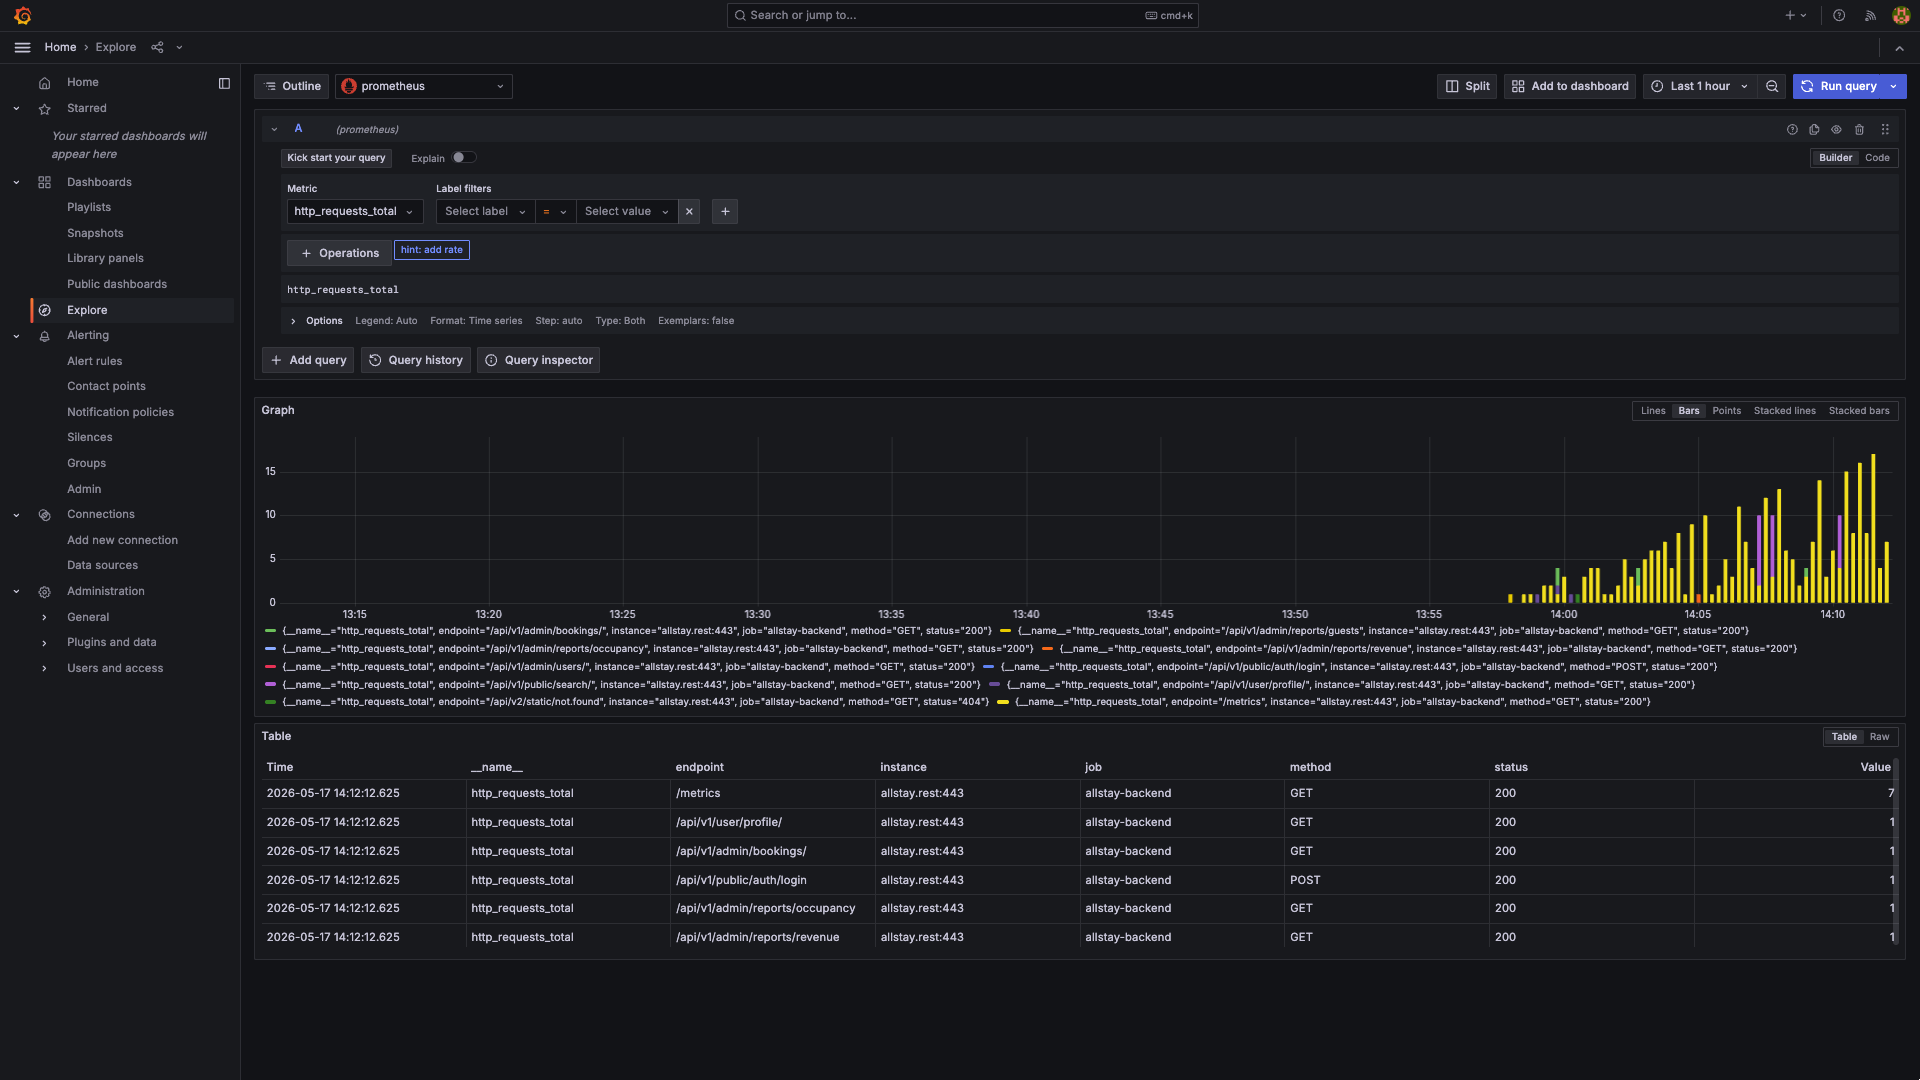
\includegraphics[width=\linewidth, height=0.38\textheight, keepaspectratio]{report_assets/grafana_http.png}
  \caption{Grafana Explore --- \texttt{http\_requests\_total} counter by endpoint, method, and status code scraped from the live production backend}
\end{figure}

\begin{figure}[H]
  \centering
  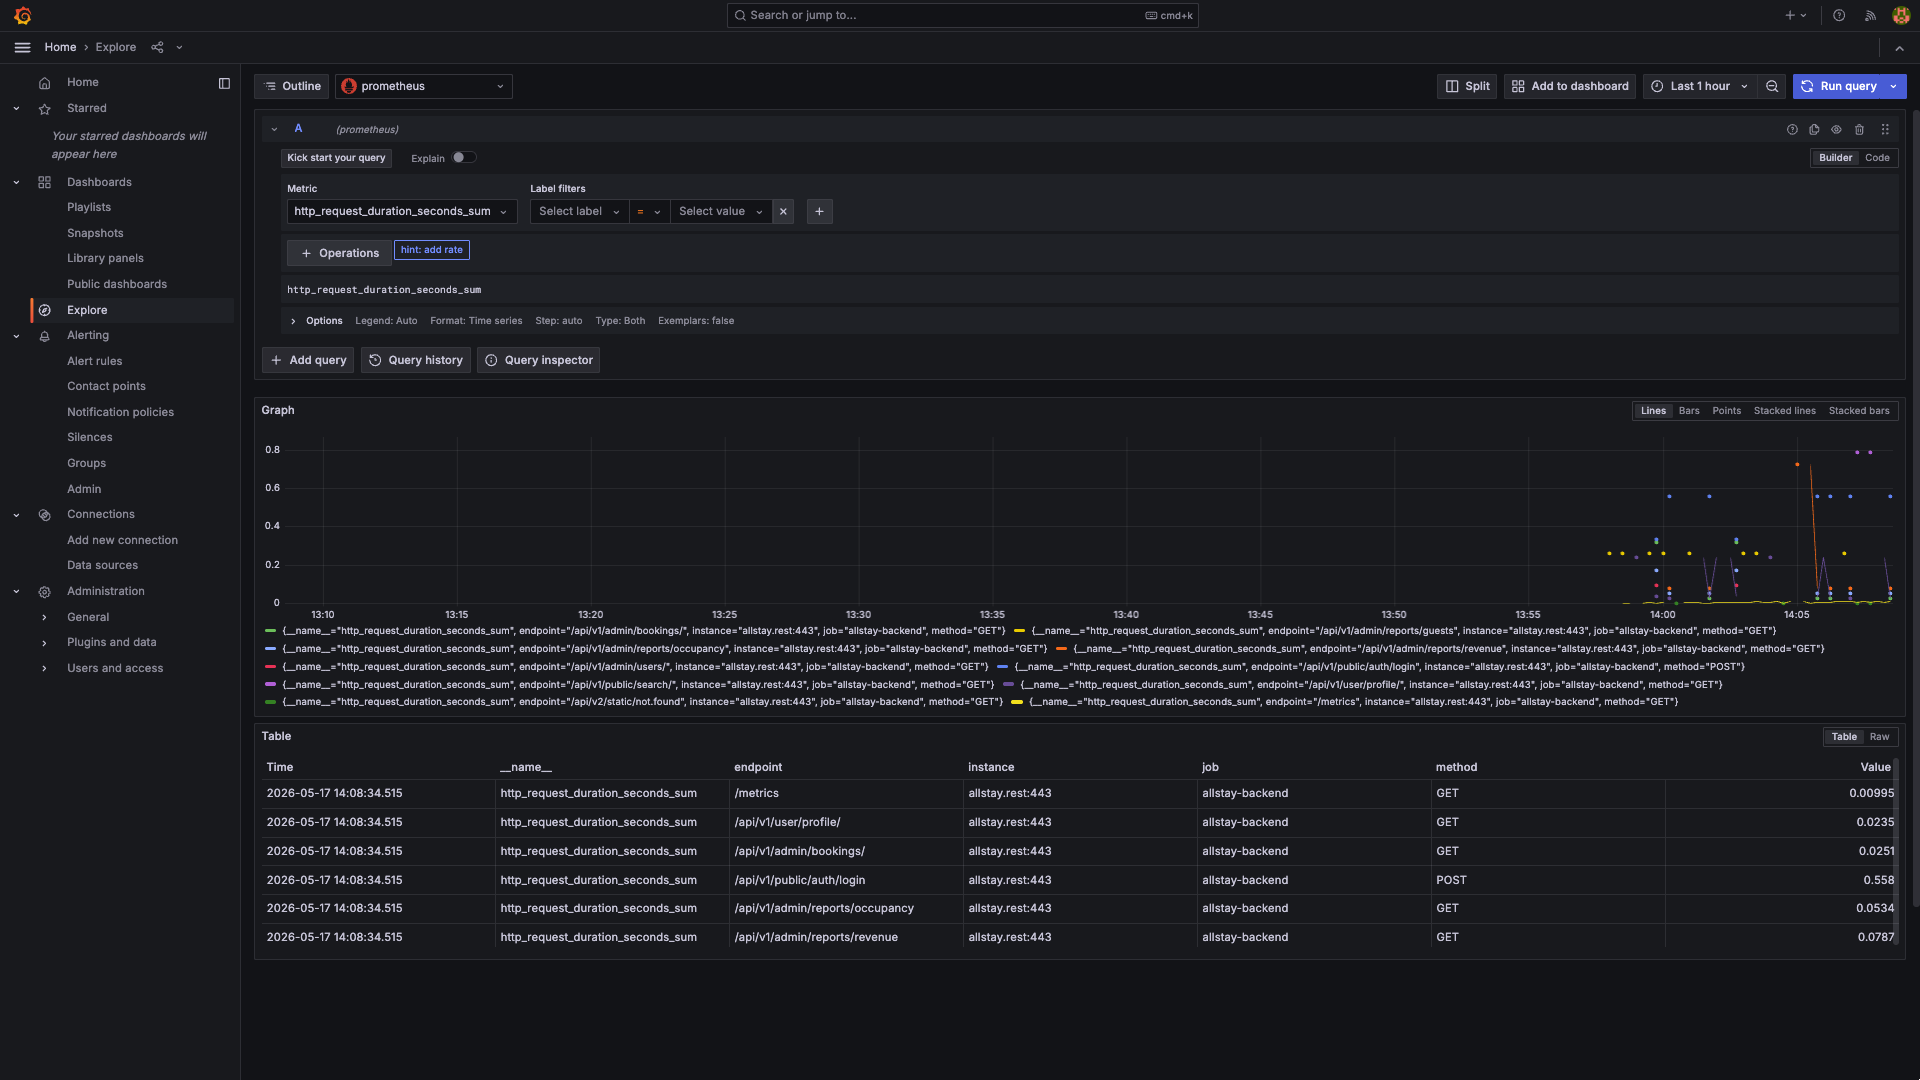
\includegraphics[width=\linewidth, height=0.38\textheight, keepaspectratio]{report_assets/grafana_latency.png}
  \caption{Grafana Explore --- \texttt{http\_request\_duration\_seconds\_sum} showing per-endpoint cumulative latency; login at $\sim$0.56\,s (includes bcrypt), profile and booking endpoints at $<$50\,ms}
\end{figure}

\begin{figure}[H]
  \centering
  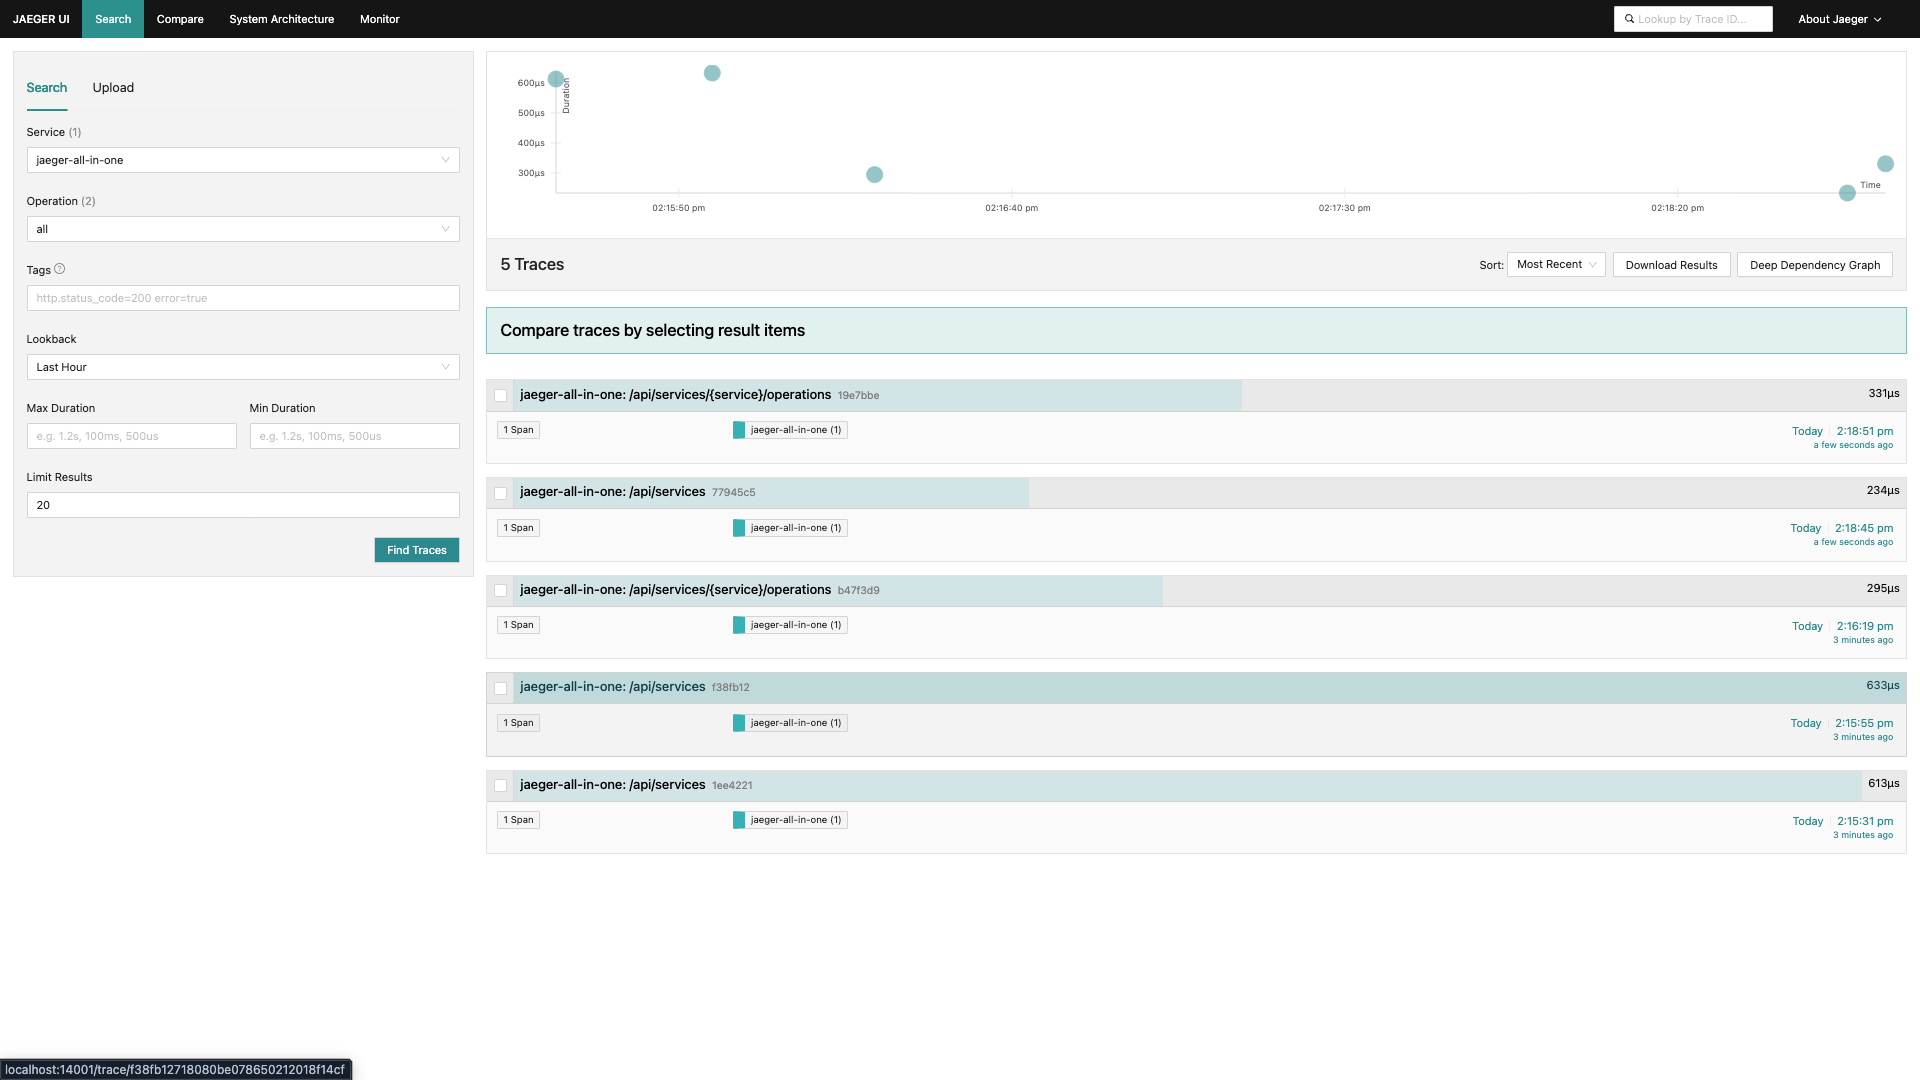
\includegraphics[width=\linewidth, height=0.38\textheight, keepaspectratio]{report_assets/jaeger_trace.png}
  \caption{Jaeger UI --- distributed trace spans exported via OTLP gRPC from \texttt{app/core/tracing.py} to Jaeger on port~4317; the waterfall view shows end-to-end request timing across service boundaries}
\end{figure}

% ══════════════════════════════════════════════════════════════════════════════
%  10. TESTING AND KNOWN LIMITATIONS
% ══════════════════════════════════════════════════════════════════════════════
\section{Testing and Known Limitations}

\subsection{Test Suite}

Integration tests live in \texttt{backend/tests/} and run with:
\begin{lstlisting}[language=bash]
cd backend && pytest tests/ -v
\end{lstlisting}

Test modules cover:
\begin{itemize}[noitemsep]
  \item \texttt{test\_auth.py} --- registration, login, token refresh, Google OAuth callback, email verification.
  \item \texttt{test\_bookings.py} --- create booking, availability guard, cancel, check-in/out.
  \item \texttt{test\_rooms.py} --- room CRUD, soft delete, availability queries.
  \item \texttt{test\_pricing.py} --- pricing rule application, priority resolution, blackout enforcement.
  \item \texttt{test\_admin.py} --- admin-only endpoints, RBAC rejection for guest tokens.
\end{itemize}

Tests use a dedicated test database (configured via \texttt{pytest.ini} and \texttt{conftest.py}) and \texttt{factories.py} for deterministic fixture data.

\subsection{Known Limitations}

\begin{itemize}[noitemsep]
  \item \textbf{Payment integration:} The payment flow records payment-intent metadata but does not integrate a real payment gateway (e.g.\ Stripe). The \texttt{payments} table stores card-method metadata only.
  \item \textbf{Single Redis node:} Token-bucket state and availability cache share one Redis instance. Redis AOF persistence mitigates crash risk, but true HA would require Redis Sentinel or Cluster.
  \item \textbf{WebSocket sticky sessions:} If the pinned replica restarts, the client must reconnect. Redis Pub/Sub handles message delivery across replicas but not automatic reconnection.
  \item \textbf{Read-replica lag:} The hot-standby replica may lag 1--2 replication cycles behind the primary; analytics reports could show slightly stale data during peak write periods.
  \item \textbf{Meilisearch index freshness:} The Celery \texttt{indexing\_tasks} re-index on hotel/room mutations. A worker crash between a write and its index update could cause a brief inconsistency window (eventual consistency).
  \item \textbf{No end-to-end frontend tests:} The React SPA is tested manually; there are no Playwright or Cypress tests at this stage.
\end{itemize}

% ══════════════════════════════════════════════════════════════════════════════
%  11. TEAM CONTRIBUTION TABLE
% ══════════════════════════════════════════════════════════════════════════════
\section{Team Contribution Table}

\begin{table}[H]
\centering\small
\begin{tabularx}{\linewidth}{@{} l l X r @{}}
\toprule
\textbf{Name} & \textbf{ID} & \textbf{Owned Features} & \textbf{Commit \%} \\
\midrule
Axmadov Sunnat & U2310044
  & System architecture, Docker Compose stack, Traefik gateway, CI/CD pipelines, Celery integration, MinIO storage, Meilisearch, project coordination
  & 35\% \\[3pt]
Mirshod Hamroyev & U2310088
  & Auth service (JWT, Google OAuth, email verification, password reset), RBAC middleware, WebSocket server and Redis Pub/Sub fan-out
  & 18\% \\[3pt]
Nurmuhammad Fazliddinov & U2310082
  & All 20 SQLAlchemy models, Alembic migration scripts, seed data, PgBouncer configuration, PostgreSQL streaming replication
  & 15\% \\[3pt]
Hamidov Abror & U2310087
  & DigitalOcean provisioning, Traefik TLS/Let's Encrypt, GitHub Actions workflows, Nginx static config, production \texttt{.env} management
  & 12\% \\[3pt]
Yusufova Muxlisa & U2310298
  & React~18 SPA --- all public, user, admin, and staff pages; Tailwind design system; i18next localisation (8~languages); AIHelper concierge chat
  & 13\% \\[3pt]
Izbosarov Bekzod & U2310113
  & Prometheus middleware, Grafana dashboards, Loki/Promtail pipeline, OpenTelemetry tracing, pytest integration test suite, token-bucket rate limiter
  & 7\% \\
\bottomrule
\end{tabularx}
\caption{Commit ratios are approximate, derived from \texttt{git shortlog -sn} on the \texttt{main} branch as of 17~May~2026.}
\end{table}

% ══════════════════════════════════════════════════════════════════════════════
%  REFERENCES
% ══════════════════════════════════════════════════════════════════════════════
\section{References}

\begin{enumerate}[leftmargin=*, label={[\arabic*]}]

\item Kleppmann, M. (2017). \textit{Designing Data-Intensive Applications}. O'Reilly Media. --- Token-bucket design (\S12), consistency models (\S\S5--9).

\item Xu, A. (2020). \textit{System Design Interview: An Insider's Guide, Vol.~1}. ByteByteGo. --- Rate limiter (Ch.~4), load balancer patterns (Ch.~1).

\item FastAPI documentation. \url{https://fastapi.tiangolo.com/} --- ASGI middleware, dependency injection, WebSocket.

\item Traefik documentation. \url{https://doc.traefik.io/traefik/} --- Dynamic configuration, Let's Encrypt, load balancing.

\item Meilisearch documentation. \url{https://www.meilisearch.com/docs/} --- Index configuration, faceted search, typo tolerance.

\item Redis documentation --- Lua scripting. \url{https://redis.io/docs/manual/programmability/lua-api/}

\item OpenTelemetry Python SDK. \url{https://opentelemetry-python.readthedocs.io/}

\item SQLAlchemy~2.0 documentation. \url{https://docs.sqlalchemy.org/en/20/} --- Async session, relationship loading.

\item Celery documentation. \url{https://docs.celeryq.dev/en/stable/} --- Beat scheduler, task serialisation.

\item PostgreSQL streaming replication. \url{https://www.postgresql.org/docs/current/warm-standby.html}

\end{enumerate}

\end{document}
